\subsection{Scenario Milestone}
\begin{figure}[H] 
    \centering 
    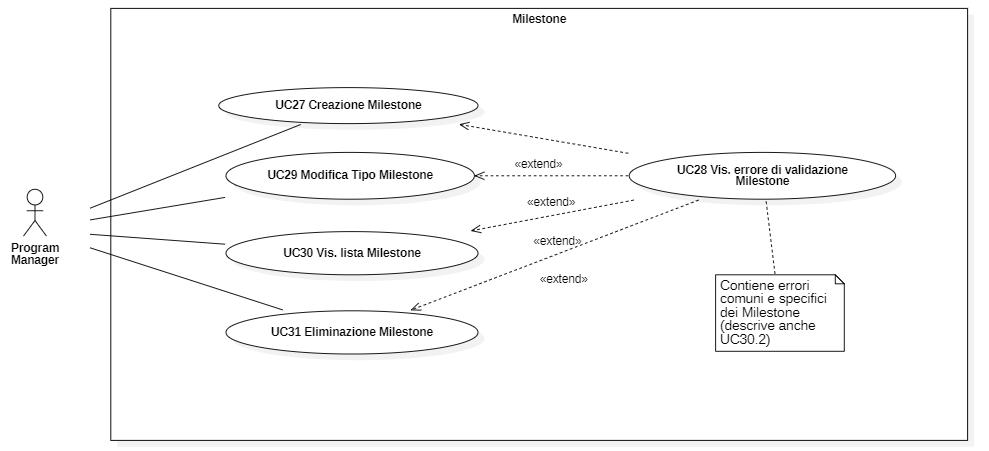
\includegraphics[width=1.1\columnwidth]{usecase/milestone-general} 
    \caption{Casi d'Uso del scenario Milestone}
\end{figure}

\subsubsection*{UC27 - Creazione Milestone}
\begin{itemize}[label=$\circ$]
\item \textbf{Attore:} Program Manager;
\item \textbf{Descrizione:} il Program Manager può creare una nuova Milestone da associare ad una Pianificazione;
\item \textbf{Precondizioni:} il richiedente è un Program Manager;
\item \textbf{Postcondizioni:} la Milestone è stata creata dal Program Manager con successo;
\item \textbf{Estensioni:} UC28;
\item \textbf{Inclusioni:} il caso d'uso non ha inclusioni.
\end{itemize}

\subsubsection*{UC28 - Vis. errore di validazione Milestone}
\begin{itemize}[label=$\circ$]
\item \textbf{Attore:} Program Manager;
\item \textbf{Descrizione:} questo caso d'uso descrive anche UC30.2. Viene visualizzato un messaggio di errore in caso vengano eseguite funzionalità con dati non validi. Esso rappresenta i seguenti errori comuni all'interno delle Milestone: dati non validi, filtri non valorizzati, entità associate non valide, risultati nulli o non valorizzati;
\item \textbf{Precondizioni:} il Program Manager sta effettuando operazioni con dati non validi;
\item \textbf{Postcondizioni:} l'esecuzione della funzionalità è interrotta e viene visualizzato il messaggio di errore;
\item \textbf{Estensioni:} il caso d'uso non ha estensioni;
\item \textbf{Inclusioni:} il caso d'uso non ha inclusioni.
\end{itemize}

\subsubsection*{UC29 - Modifica Tipo Milestone}
\begin{itemize}[label=$\circ$]
\item \textbf{Attore:} Program Manager;
\item \textbf{Descrizione:}  il Program Manager può modificare il Tipo di una Milestone in due possibili valori: Alert o Reminder;
\item \textbf{Precondizioni:} il richiedente è un Program Manager;
\item \textbf{Postcondizioni:} la Milestone è stata modificata con successo solo nel campo
Tipo dal Program Manager;
\item \textbf{Estensioni:} UC28;
\item \textbf{Inclusioni:} il caso d'uso non ha inclusioni.
\end{itemize}

\subsubsection*{UC30 - Vis. lista Milestone}
\begin{figure}[H] 
    \centering 
    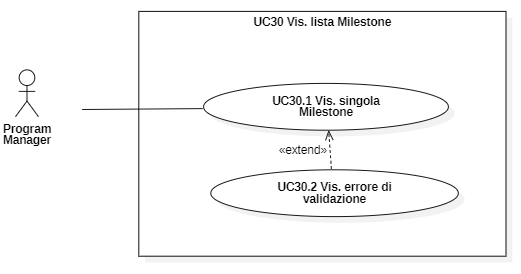
\includegraphics[width=0.70\columnwidth]{usecase/UC30} 
    \caption{Casi d'Uso 30 espanso}
\end{figure}
\begin{itemize}[label=$\circ$]
\item \textbf{Attore:} Program Manager;
\item \textbf{Descrizione:} il Program Manager può visualizzare una lista di Milestone dopo aver inserito filtri e/o una parola nella ricerca rapida e aver selezionato se i filtri applicati devono essere congiunti o disgiunti;
\item \textbf{Precondizioni:} il richiedente è un Program Manager;
\item \textbf{Postcondizioni:} la lista delle Milestone è visualizzabile dal Program Manager;
\item \textbf{Estensioni:} UC28;
\item \textbf{Inclusioni:} il caso d'uso non ha inclusioni.
\end{itemize}

\subsubsection*{UC30.1 - Vis. singola Milestone}
\begin{center}
\begin{figure}[H] 
    \centering 
    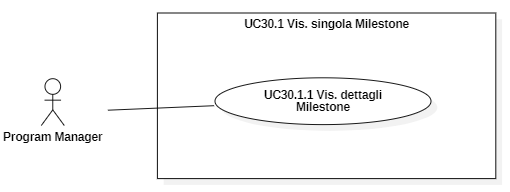
\includegraphics[width=0.70\columnwidth]{usecase/UC30.1} 
    \caption{Casi d'Uso 30.1 espanso}
\end{figure}
\end{center}
\begin{itemize}[label=$\circ$]
\item \textbf{Attore:} Program Manager;
\item \textbf{Descrizione:} il Program Manager può visualizzare la Milestone selezionata;
\item \textbf{Precondizioni:} la lista delle Milestone è visualizzabile;
\item \textbf{Postcondizioni:} la Milestone selezionata è visualizzabile dal Program Manager;
\item \textbf{Estensioni:} UC30.2;
\item \textbf{Inclusioni:} il caso d'uso non ha inclusioni.
\end{itemize}

\subsubsection*{UC30.1.1 - Vis. dettagli Milestone}
\begin{itemize}[label=$\circ$]
\item \textbf{Attore:} Program Manager;
\item \textbf{Descrizione:} il Program Manager può visualizzare la Milestone selezionata;
\item \textbf{Precondizioni:} la Milestone singola è visualizzabile;
\item \textbf{Postcondizioni:} il Project Manager può visualizzare i campi di una Milestone selezionata;
\item \textbf{Estensioni:} il caso d'uso non ha esclusioni;
\item \textbf{Inclusioni:} il caso d'uso non ha inclusioni.
\end{itemize}

\subsubsection*{UC31 - Eliminazione Milestone}
\begin{itemize}[label=$\circ$]
\item \textbf{Attore:} Program Manager;
\item \textbf{Descrizione:} il Program Manager può eliminare una Milestone esistente;
\item \textbf{Precondizioni:} il richiedente è un Program Manager;
\item \textbf{Postcondizioni:} la Milestone è stata eliminata dal Program Manager con successo;
\item \textbf{Estensioni:} UC28;
\item \textbf{Inclusioni:} il caso d'uso non ha inclusioni.
\end{itemize}